\chapter{Apêndice B — Modelos e Templates Utilizados}

Este apêndice compila todos os templates sugeridos durante o manual, permitindo
que os grupos os reutilizem sem precisar procurá-los no texto principal.

\section*{Template: Documento de Requisitos (REQ.md)}

\begin{verbatim}
	# Documento de Requisitos
	- Objetivo
	- Funcionalidades
	- User stories
	- Regras de negócio
	- Restrições
\end{verbatim}

\section*{Template: Arquitetura (ARCHITECTURE.md)}

\begin{verbatim}
	# Arquitetura
	- Visão geral
	- Componentes
	- API
	- Modelo de dados
	- Fluxos
\end{verbatim}

% ======= DIAGRAMA DE ARQUITETURA =======
\begin{figure}[ht]
	\centering
	\resizebox{\textwidth}{!}{
	\begin{tikzpicture}[
		service/.style={rectangle, draw, rounded corners=4pt, minimum width=3.6cm, minimum height=0.9cm, align=center},
		db/.style={cylinder, shape border rotate=90, aspect=0.6, draw, minimum height=1.2cm, minimum width=1.2cm},
		integ/.style={draw, ellipse, minimum width=2.2cm, minimum height=1cm},
		>=Stealth
		]
		\node[service] (ui) {Frontend\\(Web / Mobile)};
		\node[service,right=2.4cm of ui] (api) {API Gateway / Backend};
		\node[service,right=2.4cm of api] (workers) {Workers / Jobs};
		\node[db,below=1.2cm of api] (db) {Banco de Dados};
		\node[integ,below=1.2cm of workers] (mq) {Fila / Message Broker};
		
		\draw[->] (ui) -- node[above]{HTTPS / REST} (api);
		\draw[->] (api) -- node[above]{Jobs / Async} (workers);
		\draw[->] (api) -- node[right]{SQL / ORM} (db);
		\draw[->] (workers) -- node[right]{Consume / Produce} (mq);
		\draw[->] (mq) -- node[left]{Trigger} (workers);
		\end{tikzpicture}% 
	}
	\caption{Diagrama de arquitetura sugerido — separação de responsabilidades.}
\end{figure}
% ======= FIM =======

% ======= DIAGRAMA ER =======
\begin{figure}[ht]
	\centering
	\begin{tikzpicture}[
		entity/.style={rectangle, draw, minimum width=3.4cm, minimum height=1cm, align=left},
		rel/.style={draw, diamond, minimum width=1cm, inner sep=2pt}
		]
		\node[entity] (user) {Usu\'ario\\\footnotesize id\_usuario, nome, email, senha};
		\node[entity,right=3.0cm of user] (order) {Pedido\\\footnotesize id\_pedido, data, valor, id\_usuario};
		\node[entity,below=2.0cm of order] (item) {ItemPedido\\\footnotesize id\_item, id\_pedido, id\_produto, quantidade};
		\node[entity,left=3.0cm of item] (product) {Produto\\\footnotesize id\_produto, nome, preco};
		
		\draw (user) -- node[midway,above]{1 -- N} (order);
		\draw (order) -- node[midway,right]{1 -- N} (item);
		\draw (item) -- node[midway,below]{N -- 1} (product);
	\end{tikzpicture}
	\caption{Modelo ER simplificado (Usu\'ario, Pedido, Item, Produto).}
\end{figure}
% ======= FIM =======
% ======= DIAGRAMA DE SEQUÊNCIA (SIMPLIFICADO) =======
\begin{figure}[ht]
	\centering
	\begin{tikzpicture}[>=Stealth, every node/.style={font=\small}]
		% Lifelines
		\node (u) at (0,0) {Usu\'ario};
		\node (ui) at (4,0) {Frontend};
		\node (api) at (8,0) {API};
		\node (db) at (12,0) {Banco};
		
		% vertical lines
		\foreach \x in {0,4,8,12}{
			\draw (\x,-0.6) -- (\x,-6);
		}
		
		% arrows
		\draw[->] (0,-0.8) -- node[above]{preenche formul\'ario} (4,-0.8);
		\draw[->] (4,-1.4) -- node[above]{POST /login (credenciais)} (8,-1.4);
		\draw[->] (8,-2.0) -- node[above]{SELECT user WHERE email = ?} (12,-2.0);
		\draw[->] (12,-2.6) -- node[above]{row (user)} (8,-2.6);
		\draw[->] (8,-3.2) -- node[above]{200 OK + token} (4,-3.2);
		\draw[->] (4,-3.8) -- node[above]{exibe tela inicial} (0,-3.8);
		
		% notes
		\node[anchor=west] at (0.5,-5.6) {\footnotesize Observa\c{c}\%c{a}o: validar senha com hash no servidor.};
	\end{tikzpicture}
	\caption{Diagrama de sequ\'encia simplificado do fluxo de login.}
\end{figure}
% ======= FIM =======
% ======= GANTT SIMPLIFICADO (PGFPLOTS) =======
\begin{figure}[ht]
	\centering
	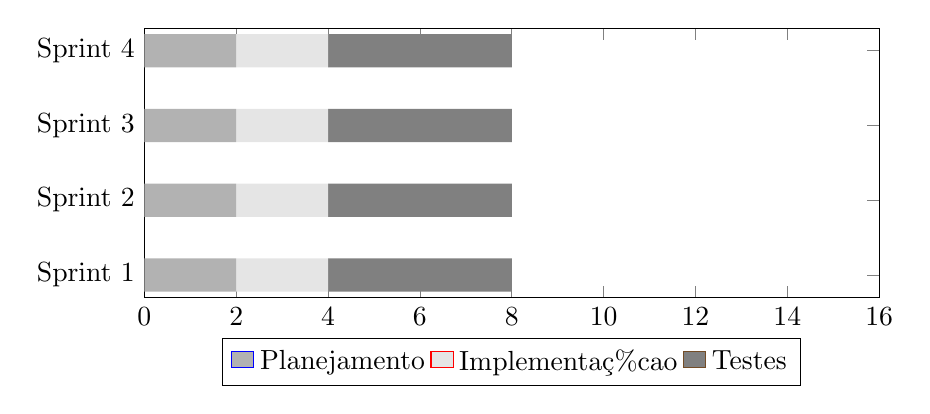
\begin{tikzpicture}
		\begin{axis}[
			xbar stacked,
			xmin=0, xmax=16,
			ytick={1,2,3,4},
			yticklabels={Sprint 1, Sprint 2, Sprint 3, Sprint 4},
			xlabel={Semanas},
			width=0.9\textwidth,
			height=5cm,
			bar width=12pt,
			legend style={at={(0.5,-0.15)},anchor=north,legend columns=3}
			]
			\addplot+[draw=none,fill=black!30] coordinates {(2,4) (2,3) (2,2) (2,1)};
			\addplot+[draw=none,fill=black!10] coordinates {(2,4) (2,3) (2,2) (2,1)};
			\addplot+[draw=none,fill=black!50] coordinates {(4,4) (4,3) (4,2) (4,1)};
			\legend{Planejamento, Implementa\c{c}\%c{a}o, Testes}
		\end{axis}
	\end{tikzpicture}
	\caption{Cronograma simplificado por sprints (exemplo). Ajuste valores conforme seu calend\'ario.}
\end{figure}
% ======= FIM =======


\section*{Template: Issue}

\begin{verbatim}
	# Descri\c{c}\%c{a}o
	# Tarefas
	# Crit\'erios de Aceita\c{c}\%c{a}o
\end{verbatim}